\chapter{Lecture 2: String Theory and M-Theory}

These notes follow Leonard Susskind's second lecture on string theory, curated in this archive by LazyingArt LLC. The lecture proceeds in a very deliberate order. First it stocks the blackboard with the interval calculus and Fourier facts that would otherwise interrupt the story later. Then it pauses over a conceptual question that matters more than it first appears to: in what sense can a string, made of many pieces, still count as a particle? Only after that does it return to the infinite-momentum or light-front point of view, build the open string as a chain of masses and springs, take the continuum limit, solve the endpoint puzzle, and quantize the resulting modes.

\section{Mathematical Preliminaries on the Interval $[0,\pi]$}

Susskind begins by saying explicitly why he is doing this: if these preliminaries were not written down now, they would have to be inserted later in the middle of the string theory, and that would be a nuisance. So we begin with the reservoir of tools.

Take a function \(x(\sigma)\) on the interval \(0\leq \sigma \leq \pi\). The choice of letters is not accidental. He uses \(x\) and \(\sigma\) because these are the notations string theory will keep returning to. The interval \([0,\pi]\) is likewise chosen in advance because it is the natural interval for the open string in this lecture.

We approximate the continuous function by values on a lattice of \(N\) points. If
\begin{equation}
\Delta \sigma=\frac{\pi}{N},
\end{equation}
then the standard replacements are
\begin{align}
x(\sigma) &\longrightarrow x_i, \\
\Delta x_i \equiv x_i-x_{i-1} &\approx \frac{\partial x}{\partial \sigma}\,\Delta \sigma, \\
\sum_i x_i\,\Delta \sigma &\longrightarrow \int_0^\pi x(\sigma)\,d\sigma .
\end{align}
This is just calculus, but it is precisely the calculus we will soon use for the string.

The next distinction is between endpoint behaviors. Here the lecture is still mathematical rather than physical, but the physical pictures are already visible.

\paragraph{Dirichlet boundary conditions.}
These fix the value of the function at the endpoints:
\begin{equation}
x(0)=x(\pi)=0.
\end{equation}
A violin string with its ends pinned down is the elementary model.

\paragraph{Neumann boundary conditions.}
These instead fix the slope at the endpoints:
\begin{equation}
\left.\frac{\partial x}{\partial \sigma}\right|_{\sigma=0}
=
\left.\frac{\partial x}{\partial \sigma}\right|_{\sigma=\pi}
=0.
\end{equation}
The function need not vanish there; it is only required to be flat.

The lecture briefly wanders through organ pipes and other examples, but the moral is simple. Dirichlet means fixed endpoints. Neumann means free endpoints. Susskind even gives a mechanical picture of a string whose ends pass through very light rings sliding on poles: not held down, but free to move. That is the kind of system for which Neumann conditions are natural.

There is also a small caution here. Piecewise continuous functions are allowed in Fourier analysis, but for the purposes of string theory we do not want jumps in the string itself: a jump would mean the string had broken.

Once the endpoint behavior is fixed, the Fourier basis is fixed with it. On \([0,\pi]\) one writes
\begin{align}
x_D(\sigma) &= \sum_{n=1}^{\infty} x_n \sin n\sigma, \\
x_N(\sigma) &= \sum_{n=0}^{\infty} x_n \cos n\sigma .
\end{align}
Sines vanish at the endpoints, which is why they go with Dirichlet. Cosines have zero derivative at the endpoints, which is why they go with Neumann. The lecture also emphasizes a fact we will use later without apology: differentiation swaps the two classes. The derivative of a Dirichlet function is Neumann; the derivative of a Neumann function is Dirichlet.

To make these expansions useful, we need the orthogonality integrals. In the form relevant later,
\begin{align}
\int_0^\pi \cos n\sigma \cos m\sigma\,d\sigma &= 0 \qquad (n\neq m), \\
\int_0^\pi \cos^2 n\sigma\,d\sigma &= \frac{\pi}{2} \qquad (n\geq 1), \\
\int_0^\pi d\sigma &= \pi, \\
\int_0^\pi \sin n\sigma \sin m\sigma\,d\sigma &= \frac{\pi}{2}\delta_{nm} \qquad (n,m\geq 1).
\end{align}

\begin{remark}
The transcript becomes garbled around the exceptional \(n=0\) cosine mode, but the intended mathematics is clear. The nonzero cosine modes have norm \(\pi/2\), while the constant mode \(\cos 0\sigma=1\) integrates to \(\pi\).
\end{remark}

The last item placed on the board is the harmonic oscillator. After rescaling the coordinate so that the mass is one, the energy reads
\begin{equation}
E_{\mathrm{osc}}=\frac{1}{2}\dot x^{\,2}+\frac{1}{2}\omega^2 x^2,
\end{equation}
and the corresponding Lagrangian is
\begin{equation}
L_{\mathrm{osc}}=\frac{1}{2}\dot x^{\,2}-\frac{1}{2}\omega^2 x^2.
\end{equation}
The lecture contains a verbal slip here, but the mathematics is standard: the Lagrangian is \(T-V\), not ``kinetic energy squared minus potential energy squared.'' The quantum fact we keep in reserve is that oscillator levels come in steps of \(\omega\), up to the overall ground-state offset.

\section{What Makes a String a Particle?}

Now the lecture deliberately interrupts its own mathematical flow. Before building the string, it asks a question that could otherwise become a source of confusion for the rest of the course: what do we mean by a particle at all?

A string, after all, is about to be modeled as a large number of pieces connected by springs. If that is so, why should it behave like a particle rather than like an ordinary extended object?

The first part of the answer is negative. Pointlikeness is not the criterion. Electrons are surrounded by virtual clouds. Protons and neutrons are obviously composite. The lecture insists that what we call a particle need not be literally structureless.

Nor is it enough merely to have a mass and a center-of-mass position. A box of gas has those. A cup of coffee has those. Yet no physicist would naturally call a cup of coffee a particle.

\subsection{Question \& Answer}

\paragraph{Question.}
When does a composite object count as a particle rather than ``mush''?

\paragraph{Answer.}
A composite object counts as a particle when the excitation spectrum above its ground state is discrete and well separated. If there are large enough gaps to the first few excited states, the object behaves as an isolated quantum species. If instead there are innumerable nearby states at arbitrarily small separations, the object behaves like continuum matter.

This is the lesson of the lecture's coffee example. A cup of coffee can be excited by tiny disturbances: one can stir it slightly, excite a sound mode, disturb a molecule, or create a phonon with an absurdly small amount of energy. The nearby states are so dense that they practically form a continuum. That is mush.

A proton is different. It certainly has excitations, but it takes a substantial amount of energy to get to them. The nearby spectrum is not continuous. An electron is more isolated still. One does not have a ladder of electron states lying immediately above the electron.

So the criterion becomes spectral rather than ontological. The question for string theory is not whether the string is made of parts. Of course it is. The question is whether the internal excitations are separated by large enough gaps to make the lowest state behave as a particle. In the version of string theory under discussion, the gap is taken to be enormous, on the scale of the Planck mass, and that is why the string may still present itself as a particle in ordinary experiments.

This detour is not philosophical ornament. It prepares the central claim of the lecture's last third: once the string is quantized, its spectrum comes out discrete enough to justify calling the resulting states particles.

\section{Review of the Infinite-Momentum / Light-Front Trick}

Only after that conceptual pause does Susskind return to the framework from the previous lecture. The question is this: how can an extended relativistic system ever be described by something as simple as nonrelativistic mechanics?

He first emphasizes what does \emph{not} work. A rapidly spinning baton is not well described by nonrelativistic physics just because we happen to sit in the frame where its center of mass is simple. The issue is the relative motion of its parts. If the ends are moving relativistically relative to each other, then the ordinary nonrelativistic approximation fails.

The trick is different. We boost the whole system to a very large momentum along some chosen axis, say the \(z\)-axis, and then examine only the motion in the transverse plane. In that description the transverse dynamics become exactly, not approximately, nonrelativistic in form.

Start from the relativistic energy
\begin{equation}
E=\sqrt{P_z^2+p_x^2+p_y^2+M^2},
\end{equation}
where \(M\) is the rest mass of the full system and \(P_z\) is the large longitudinal momentum. When \(P_z\) is the dominant scale, we expand:
\begin{equation}
E \approx P_z+\frac{p_x^2+p_y^2+M^2}{2P_z}.
\end{equation}
The first term is the trivial boost energy. It depends on the conserved longitudinal momentum but not on the internal state, so for the questions at hand we subtract it and write
\begin{equation}
E-P_z=\frac{p_x^2+p_y^2+M^2}{2P_z}.
\end{equation}

The lecture then makes the crucial interpretive move. Energy is Hamiltonian. Hamiltonian governs time evolution. But if \(P_z\) becomes very large, the right-hand side tends to zero, which means that in the ordinary time variable the internal motion appears to freeze. This is just time dilation.

We do not want to throw away the internal motion. We want to follow it. So we rescale time. Equivalently, up to a conventional overall normalization, we multiply by \(P_z\). Then the expression has a finite limit:
\begin{equation}
P_z(E-P_z)=\frac{1}{2}\left(p_x^2+p_y^2+M^2\right).
\end{equation}
This now looks like a two-dimensional nonrelativistic Hamiltonian: transverse momentum squared divided by two, plus an internal contribution. The only conceptual twist is that the internal contribution is proportional to \(M^2\), not \(M\).

\begin{figure}[htbp]
\centering

\includegraphics[width=0.72\textwidth]{lecture_02_figure_02.png}
\caption{Hamiltonian form of the boosted energy. The board line beginning with \(H=\) marks the shift from the boosted-energy expansion to its Hamiltonian interpretation.}
\label{fig:lecture02-lightfront}
\end{figure}

On the board, the line beginning with \(H=\) records exactly this reinterpretation. The board itself does not finish writing \(H=i\,d/dt\), but the lecture makes that identification in words: Hamiltonian is what governs time evolution.

\begin{remark}
Susskind briefly complains about the terminology ``light cone'' and says that ``light front'' would be better. We keep only the mathematical point. After the large boost and the time rescaling, the transverse dynamics are exactly nonrelativistic in form.
\end{remark}

There is one more feature he flags, without dwelling on it. For strings, the longitudinal internal motion is constrained by the transverse motion. That is part of what makes the method so powerful. In the present lecture, however, this remains background motivation; the active calculation now moves to the transverse coordinates alone.

\section{A String as Mass Points and Springs}

Now we come to strings themselves. In the boosted description the string moves only in two transverse directions, which we call \(X\) and \(Y\). The lecture begins with the discrete model: \(N\) mass points joined by \(N-1\) springs.

The coordinate \(\sigma\) labels position along the string and runs from \(0\) to \(\pi\). This is not forced; it is chosen. Susskind even remarks that one could equally well choose \(0\) to \(1\) or \(0\) to \(2\). The reason for choosing \([0,\pi]\) is pedagogical. He wants to reserve \([0,2\pi]\) for the closed string later on.

The discrete energy of the open string is
\begin{equation}
E=\sum_i\left[
\frac{\mu}{2}\bigl(\dot X_i^2+\dot Y_i^2\bigr)
+
\frac{k}{2}\bigl((\Delta X_i)^2+(\Delta Y_i)^2\bigr)
\right].
\end{equation}
The board writes the bead mass as \(m\), but the lecture itself later corrects this and introduces \(\mu\) as the nonrelativistic analog mass of each bead, so we use \(\mu\) from the start in the cleaned notes. Likewise, the spring constant is called both \(k\) and \(\kappa\) in speech; we write \(k\).

\begin{figure}[htbp]
\centering

\includegraphics[width=0.72\textwidth]{lecture_02_figure_03.png}
\caption{Discrete string as mass points and springs. The lecture moves directly from the bead-chain sketch to the discrete energy formula.}
\label{fig:lecture02-discrete-board}
\end{figure}

\begin{figure}[htbp]
\centering
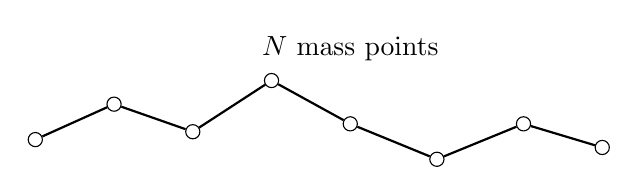
\begin{tikzpicture}[scale=1.0]
\draw[thick] (0,0) -- (1.0,0.45) -- (2.0,0.10) -- (3.0,0.75) -- (4.0,0.20) -- (5.1,-0.25) -- (6.2,0.20) -- (7.2,-0.10);
\foreach \x/\y in {0/0,1.0/0.45,2.0/0.10,3.0/0.75,4.0/0.20,5.1/-0.25,6.2/0.20,7.2/-0.10}
{
  \filldraw[white] (\x,\y) circle (0.09);
  \draw (\x,\y) circle (0.09);
}
\node at (4.0,1.15) {$N$ mass points};
\end{tikzpicture}
\caption{A clean redraw of the bead-chain model used to take the continuum limit.}
\label{fig:lecture02-discrete-tikz}
\end{figure}

When Susskind writes the formula first for \(X\), he immediately says: wherever I write \(X\), you must also add the same thing with \(Y\). That small spoken reminder matters. The string lives in two transverse directions, not one.

The next task is to choose the large-\(N\) scaling correctly. If the number of beads grows while each bead keeps a fixed mass, then the total mass diverges. That is not the continuum limit we want. We therefore choose
\begin{equation}
\mu=\frac{1}{N},
\end{equation}
so that the total analog mass remains fixed.

The spring constant must scale in the opposite direction. Springs in series make a long chain easier to stretch, so if the overall stiffness of the string is to stay finite, the microscopic springs must become stiffer as the chain is refined. Susskind chooses
\begin{equation}
k=\frac{N}{\pi^2}.
\end{equation}
The factor of \(\pi^2\) is a convention inserted only to simplify later formulas. The essential point is the \(k\sim N\) scaling.

This is the real payoff of the opening calculus detour. We now have a discrete mechanical chain and a precise prescription for taking its continuum limit.

\section{Continuum Energy, Lagrangian, and Wave Interpretation}

At this point the lecture uses, almost verbatim, the formulas it put on the board at the beginning. We have \(\Delta \sigma=\pi/N\), we have sums, and we have nearest-neighbor differences. Now we turn them into integrals and derivatives.

\paragraph{A worked derivation of the continuum limit.}
For the \(X\)-sector kinetic term,
\begin{align}
\sum_i \frac{\mu}{2}\dot X_i^2
&=
\sum_i \frac{1}{2N}\dot X_i^2 \\
&=
\frac{1}{2\pi}\sum_i \dot X_i^2\,\Delta \sigma \\
&\longrightarrow
\frac{1}{2\pi}\int_0^\pi d\sigma
\left(\frac{\partial X}{\partial \tau}\right)^2.
\end{align}
For the spring term we use the continuum replacement
\begin{equation}
\Delta X_i \approx \frac{\partial X}{\partial \sigma}\,\Delta \sigma.
\end{equation}
Then
\begin{align}
\sum_i \frac{k}{2}(\Delta X_i)^2
&\approx
\sum_i \frac{N}{2\pi^2}
\left(\frac{\partial X}{\partial \sigma}\right)^2
(\Delta \sigma)^2 \\
&=
\sum_i \frac{1}{2N}
\left(\frac{\partial X}{\partial \sigma}\right)^2 \\
&=
\frac{1}{2\pi}\sum_i
\left(\frac{\partial X}{\partial \sigma}\right)^2
\Delta \sigma \\
&\longrightarrow
\frac{1}{2\pi}\int_0^\pi d\sigma
\left(\frac{\partial X}{\partial \sigma}\right)^2.
\end{align}
Exactly the same steps apply to \(Y\).

So the continuum energy becomes
\begin{equation}
E=
\frac{1}{2\pi}\int_0^\pi d\sigma
\left[
\left(\frac{\partial X}{\partial \tau}\right)^2
+
\left(\frac{\partial Y}{\partial \tau}\right)^2
+
\left(\frac{\partial X}{\partial \sigma}\right)^2
+
\left(\frac{\partial Y}{\partial \sigma}\right)^2
\right],
\end{equation}
and the continuum Lagrangian is
\begin{equation}
L=
\frac{1}{2\pi}\int_0^\pi d\sigma
\left[
\left(\frac{\partial X}{\partial \tau}\right)^2
+
\left(\frac{\partial Y}{\partial \tau}\right)^2
-
\left(\frac{\partial X}{\partial \sigma}\right)^2
-
\left(\frac{\partial Y}{\partial \sigma}\right)^2
\right].
\end{equation}

\begin{figure}[htbp]
\centering

\includegraphics[width=0.76\textwidth]{lecture_02_figure_04.png}
\caption{Continuum string Lagrangian. The board records the moment at which the minus sign of the potential term is being written.}
\label{fig:lecture02-continuum}
\end{figure}

The lecture pauses here to make an illuminating comparison. If we rename \(\sigma\) as a spatial coordinate on a line and rename \(X\) as a field \(\phi\), then this is just the energy of an ordinary wave system. Waves move left and right along the interval. When they hit the boundary, they reflect.

The boundary condition determines the character of the reflection. Under Dirichlet conditions the reflected wave flips sign. Under Neumann conditions it reflects without such inversion. Susskind says one could now write down the wave equation by varying the Lagrangian, but refuses to do so because the lecture will not need it. That refusal is part of the rhythm of the presentation, and we keep it. The wave viewpoint is useful; the full partial differential equation is not yet needed.

One more spoken clarification belongs here. The time variable \(\tau\) is the rescaled time appropriate to the boosted description. Susskind loosely calls it proper time: the time carried along by the boosted clock so that we can continue to watch the internal motion instead of letting it freeze under time dilation.

Finally, the lecture reminds us why this energy matters. In the light-front description, the internal energy of the string will be identified, up to the same overall normalization convention as before, with the square of the relativistic mass of the string state.

\section{Endpoint Dynamics and the Boundary-Condition Puzzle}

Now the lecture returns to a question it deliberately postponed earlier. We have seen both Dirichlet and Neumann conditions. We have heard that free string endpoints should obey Neumann conditions. Why?

Here the lecture is at its cleanest. It raises the obstacle plainly and resolves it with a short Newton-law argument.

\begin{figure}[htbp]
\centering

\includegraphics[width=0.68\textwidth]{lecture_02_figure_05.png}
\caption{Discrete difference becomes derivative times spacing. This is the local step that converts the endpoint force into a boundary condition.}
\label{fig:lecture02-endpoint-board}
\end{figure}

\begin{figure}[htbp]
\centering
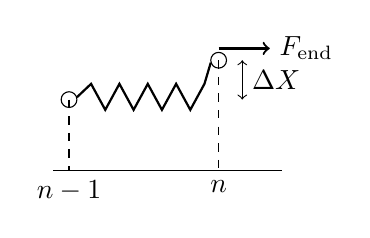
\begin{tikzpicture}[scale=1.0]
\draw[thin] (-0.2,-0.8) -- (2.7,-0.8);
\filldraw[white] (0,0.10) circle (0.10);
\draw (0,0.10) circle (0.10);
\filldraw[white] (1.9,0.60) circle (0.10);
\draw (1.9,0.60) circle (0.10);
\draw[thick]
(0.10,0.13) -- (0.28,0.30) -- (0.46,-0.03) -- (0.64,0.30) -- (0.82,-0.03) -- (1.00,0.30) -- (1.18,-0.03) -- (1.36,0.30) -- (1.54,-0.03) -- (1.72,0.30) -- (1.80,0.57);
\draw[dashed] (0,0.10) -- (0,-0.8);
\draw[dashed] (1.9,0.60) -- (1.9,-0.8);
\node[below] at (0,-0.8) {$n-1$};
\node[below] at (1.9,-0.8) {$n$};
\draw[<->] (2.2,0.10) -- (2.2,0.60);
\node[right] at (2.2,0.35) {$\Delta X$};
\draw[->,thick] (1.9,0.75) -- (2.55,0.75);
\node[right] at (2.55,0.75) {$F_{\mathrm{end}}$};
\end{tikzpicture}
\caption{Endpoint geometry for the Newton-law argument. The last mass point feels a force from only one spring.}
\label{fig:lecture02-endpoint-tikz}
\end{figure}

\subsection{Question \& Answer}

\paragraph{Question.}
Why must the open-string endpoint satisfy Neumann rather than Dirichlet boundary conditions?

\paragraph{Answer.}
Because the endpoint is free rather than pinned, and for a free endpoint Newton's law forces the local stretch to vanish in the continuum limit.

Let the last bead be labeled \(n\), and the previous one \(n-1\). An interior bead is pulled from both sides. The endpoint is special: it feels only the force from the spring connecting it to the rest of the string. By Hooke's law,
\begin{equation}
F_{\mathrm{end}}\sim k\,\Delta X.
\end{equation}
Now we use the continuum replacement that the board is capturing:
\begin{equation}
\Delta X=\frac{\partial X}{\partial \sigma}\,\Delta \sigma.
\end{equation}
Since \(k\sim N\) and \(\Delta \sigma\sim 1/N\), the \(N\)-dependence cancels, so
\begin{equation}
F_{\mathrm{end}}\propto \frac{\partial X}{\partial \sigma}.
\end{equation}
That is already the key step: the endpoint force is proportional to the slope of the string at the endpoint.

But Newton's law also says
\begin{equation}
F_{\mathrm{end}}=\mu\,\frac{\partial^2 X}{\partial \tau^2},
\qquad
\mu\sim \frac{1}{N}.
\end{equation}
So if \(\partial_\sigma X\) were nonzero at the endpoint, then the acceleration \(\partial_\tau^2 X\) would grow like \(N\) as the continuum limit is taken. The endpoint would acquire an infinite acceleration. That is exactly the pathology the lecture wants to exclude.

The cure is immediate:
\begin{equation}
\left.\frac{\partial X}{\partial \sigma}\right|_{\sigma=0,\pi}=0.
\end{equation}
And the same argument applies to \(Y\). Thus the free open-string endpoint satisfies Neumann boundary conditions.

This is a good example of the lecture's style. A boundary condition that could have been postulated as a formal rule is instead derived from a local mechanical argument. The mathematics is light, but the motivation is precise.

\section{Fourier Modes, Harmonic Oscillators, and the First Quantum Spectrum}

Now the system is finally ready to quantize. The first step is not yet quantum mechanics; it is a re-description of the classical string in terms of its harmonics.

Because the open string obeys Neumann conditions, we expand in cosines:
\begin{equation}
X(\sigma,\tau)=\sum_{n=0}^{\infty} X_n(\tau)\cos n\sigma,
\qquad
Y(\sigma,\tau)=\sum_{n=0}^{\infty} Y_n(\tau)\cos n\sigma.
\end{equation}
The dependence on \(\sigma\) is carried by the cosines. The dependence on time \(\tau\) sits in the coefficients \(X_n(\tau)\) and \(Y_n(\tau)\). That is where the string wiggles.

Differentiating with respect to time gives
\begin{equation}
\dot X(\sigma,\tau)=\sum_{n=0}^{\infty}\dot X_n(\tau)\cos n\sigma,
\end{equation}
while differentiating with respect to \(\sigma\) gives
\begin{equation}
\frac{\partial X}{\partial \sigma}
=
-\sum_{n=1}^{\infty} n\,X_n(\tau)\sin n\sigma .
\end{equation}
The board image suggests a sum beginning at \(n=0\), but the cleaned expression must begin at \(n=1\), since the differentiated zero mode vanishes.

\begin{figure}[htbp]
\centering

\includegraphics[width=0.70\textwidth]{lecture_02_figure_06.png}
\caption{Mode expansion of the \(\sigma\)-derivative. The visible board evidence is the minus sign, the factor of \(n\), and the passage from cosines to sines.}
\label{fig:lecture02-modes}
\end{figure}

Now we insert the mode expansions into the energy. This is where the orthogonality formulas from the beginning of the lecture are harvested. All cross-terms with \(n\neq m\) vanish after integration over \(\sigma\). The double sums collapse to single sums. The \(n=0\) mode must be handled separately because its cosine norm is \(\pi\) rather than \(\pi/2\).

For the kinetic piece of the \(X\)-sector we find
\begin{equation}
\frac{1}{2\pi}\int_0^\pi d\sigma\,\dot X^2
=
\frac{1}{2}\dot X_0^{\,2}
+
\frac{1}{4}\sum_{n=1}^{\infty}\dot X_n^{\,2},
\end{equation}
and for the stretching piece,
\begin{equation}
\frac{1}{2\pi}\int_0^\pi d\sigma
\left(\frac{\partial X}{\partial \sigma}\right)^2
=
\frac{1}{4}\sum_{n=1}^{\infty}n^2X_n^{\,2}.
\end{equation}
So the full \(X\)-sector energy is
\begin{equation}
E_X=
\frac{1}{2}\dot X_0^{\,2}
+
\frac{1}{4}\sum_{n=1}^{\infty}
\left(
\dot X_n^{\,2}+n^2X_n^{\,2}
\right),
\end{equation}
and the corresponding \(X\)-sector Lagrangian is
\begin{equation}
L_X=
\frac{1}{2}\dot X_0^{\,2}
+
\frac{1}{4}\sum_{n=1}^{\infty}
\left(
\dot X_n^{\,2}-n^2X_n^{\,2}
\right).
\end{equation}
The \(Y\)-sector is identical:
\begin{equation}
L_Y=
\frac{1}{2}\dot Y_0^{\,2}
+
\frac{1}{4}\sum_{n=1}^{\infty}
\left(
\dot Y_n^{\,2}-n^2Y_n^{\,2}
\right).
\end{equation}

Several things are now visible at once.

First, \(X_0\) and \(Y_0\) are the average positions of the string, hence the center-of-mass coordinates. They have kinetic energy but no restoring force. The zero mode is a free particle mode, not an oscillator.

Second, each mode with \(n\geq 1\) is an ordinary harmonic oscillator. Comparing with the earlier oscillator formula, we read off
\begin{equation}
\omega_n=n,
\qquad
n\geq 1.
\end{equation}
So the open string is a countable infinity of independent oscillators in the \(X\)-direction, together with another countable infinity in the \(Y\)-direction. These are nothing but the harmonics of the string.

Third, the internal vibrational energy is
\begin{equation}
E_{\mathrm{int}}
=
\frac{1}{4}\sum_{n=1}^{\infty}
\left(
\dot X_n^{\,2}+n^2X_n^{\,2}
+
\dot Y_n^{\,2}+n^2Y_n^{\,2}
\right).
\end{equation}
Up to the same light-front normalization convention introduced earlier, this is the quantity that becomes the relativistic mass squared of the string state. That is the bridge from oscillator mathematics back to particle physics.

Quantization is now easy. The lecture does not yet introduce creation and annihilation operators systematically; it merely uses the oscillator spectrum. For the \(n\)-th oscillator, if \(Q_n\) quanta are present and \(\hbar=1\), then the excitation energy above the unspecified ground-state offset is
\begin{equation}
\Delta E_n = Q_n\,\omega_n = Q_n\,n.
\end{equation}
Susskind is careful to rename the occupation number \(Q\) so that it is not confused with the mode label \(n\).

The lowest levels can then be counted directly.

\paragraph{Ground state.}
All oscillators are in their lowest state. This is not empty space. It is one open string with no internal excitation.

\paragraph{First excited level.}
Excite the \(n=1\) oscillator once. One may do this in the \(X\)-tower or in the \(Y\)-tower, so the first excited level has multiplicity \(2\).

\paragraph{Second excited level.}
Now the total excitation energy is \(2\). There are five possibilities:
\begin{itemize}
\item two quanta in the \(n=1\) \(X\)-oscillator,
\item two quanta in the \(n=1\) \(Y\)-oscillator,
\item one quantum in each of the \(n=1\) \(X\)- and \(Y\)-oscillators,
\item one quantum in the \(n=2\) \(X\)-oscillator,
\item one quantum in the \(n=2\) \(Y\)-oscillator.
\end{itemize}
So the second excited level has multiplicity \(5\).

This is exactly the point the lecture wanted to set up from the beginning. The open string has a discrete spectrum with appreciable gaps. It therefore behaves like a particle in the precise spectral sense explained earlier.

The final remarks of the lecture are a preview, not a full development. Open strings have endpoints, and once interactions are allowed, endpoints can join and split. A fluctuating open string may bring one of its endpoints into contact with another endpoint and thereby produce a closed string. So one may consistently have a theory of closed strings without open strings, but not a theory of open strings without closed strings. As a rough guide only, the lecture says that open strings often behave like photons, while closed strings behave like gravitons.

\section{Summary}

The lecture unfolds by preparation, obstacle, and payoff. It first stocks the blackboard with the mathematics of functions on \([0,\pi]\): discretization, boundary conditions, Fourier expansions, orthogonality, and the harmonic oscillator. It then sharpens the notion of a particle by replacing pointlikeness with spectral isolation. With that conceptual and mathematical groundwork in place, the infinite-momentum or light-front viewpoint recasts the relativistic string as an exact two-dimensional mechanical system. The open string is built as a chain of masses and springs, passed to a continuum description, fixed by a Neumann endpoint condition derived from Newton's law, and finally rewritten as an infinite collection of uncoupled harmonic oscillators. The resulting spectrum is discrete, gapped, and therefore particle-like. That is the central gain of the lecture, and it is the point from which the next step, the closed string, naturally begins.